%%%%%%%%%%%%%%%%%%%%%%%%%%%%%%%%%%%%%%%%%%%%%%%%%%%%%%%%%%%%%
%% Licensed under CC-BY
%% Original Template written by Prof. Kilu von Prince for the Department of General Linguistics at HHU Düsseldorf
%%%%%%%%%%%%%%%%%%%%%%%%%%%%%%%%%%%%%%%%%%%%%%%%%%%%%%%%%%%%%
%% English adaption for the Institute of English and American Studies by Anh Kim Nguyen and Akhilesh Kakolu Ramarao
%%%%%%%%%%%%%%%%%%%%%%%%%%%%%%%%%%%%%%%%%%%%%%%%%%%%%%%%%%%%%
%% This template is supposed to provide the most common tools needed to format a linguistic paper. Examples may be adapted, replaced, copied or deleted as the student needs them
%%%%%%%%%%%%%%%%%%%%%%%%%%%%%%%%%%%%%%%%%%%%%%%%%%%%%%%%%%%%%

\documentclass{article}
\usepackage[british]{babel}% Makes the template English, use 'american' when preferring US English

\usepackage{fontspec} % Use XeLateX when compiling with this, unless your work contains more than Unicode characters, this will be fine. If using non-Unicode characters, comment this out and use LuaLatex
\setmainfont{Linux Libertine O} % Great variety in Unicode characters, has phonetic symbols
\usepackage[margin=3cm]{geometry}

%% PACKAGES FOR FORMATTING %%%%%%%%%%%%%%%%%%%%%%%%%%%%%%%%%%

% \usepackage{linguex} % package for glossing alternative to gb4e below
\usepackage{paralist} % compact lists
\usepackage{booktabs} % add horizontal lines to your tables
\usepackage{array} % more format options for your tables
\usepackage{csquotes} % more control over quotation marks
\usepackage{float} % more control over float objects

%% CITATION, USER FRIENDLY BUT RESTRICTING %%%%%%%%%%%%%%%%%%

\usepackage{natbib}% easy to use citation style with default implementation of APA.
%% Use commands \citet{BIBKEY}, \citep[e.g][PAGE]{BIBKEY} to cite
 	\setcitestyle{notesep=:\,} % custom seperator for page numbers
%% CITATION, USER DEFINABLE %%%%%%%%%%%%%%%%%%%%%%%%%%%%%%%%%
% \usepackage[style=apa,backend=biber,useibid=true]{biblatex}

%% PACKAGES FOR COLOURING AND GRAPHICS %%%%%%%%%%%%%%%%%%%%%%

\usepackage{xcolor} 
\definecolor{HHUBlue}{RGB}{0,106,179} % Corporate Design colours of HHU
\usepackage[colorlinks=true, linkcolor=HHUBlue!70!black,citecolor=HHUBlue!80!black,urlcolor=HHUBlue!80!black]{hyperref} % Link colour in-text

\usepackage{tabularx} % Much better tables than the standard tabular
\usepackage{graphicx} % Better package for adding images
\usepackage{forest} % Syntax trees, alternatively you can use qtree, xyling
\usepackage{fancyvrb} % lets you use the "verbatim" environment, easier use of the type-writery look of text

%% Extra %%%%%%%%%%%%%%%%%%%%%%%%%%%%%%%%%%%%%%%%%%%%%%%%%%%%
\usepackage{lipsum}% lorem ipsum generator, if you just need to fill paragraphs and see if the format looks good
\usepackage{tikz-dependency} % If you need to draw dependency structures

\usepackage{gb4e} % Sentence glossings. Do not add more packages below this one, or it will break. Feel free to add packages above it
    \let\eachwordone=\itshape % Makes original sentence cursive

%%%%%%%%%%%%%%%%%%%%%%%%%%%%%%%%%%%%%%%%%%%%%%%%%%%%%%%%%%%%%%%%%%%%%%%%%%%%%%
%% BEGINNING OF DOCUMENT
%%%%%%%%%%%%%%%%%%%%%%%%%%%%%%%%%%%%%%%%%%%%%%%%%%%%%%%%%%%%%%%%%%%%%%%%%%%%%%

\begin{document}

\begin{titlepage}
\noindent\parbox{.5\textwidth}{
Institute of English and American Studies\\
Heinrich-Heine-Universität Düsseldorf\\
NAME OF CLASS\\
NAME OF TEACHER\\
SEMESTER SEASON AND YEAR}

\vfill

{\centering\Large

This is a title

}

\vfill

\noindent\parbox{.5\textwidth}
{NAME\\
STUDENT NUMBER\\
MAIL ADDRESS\\
NUMBER OF SEMESTER\\
DATE OF SUBMISSION}

\end{titlepage}

\tableofcontents

\section{Introduction}
Text for your introduction.

\section{Main}
Examples on how to use the different packages: 

\subsection{Example sentences and glossings}

\begin{exe}
\ex This is an example sentence

\ex \begin{xlista}  
\ex One example sentence 
  \ex Two example sentences
\end{xlista}


\ex \gll verdaustig war's und glasse Wieben rotterten gorkicht im Gemank\\
        brilly t'was and slithy toves gyre gymbly in.the wabe\\
        \enquote{t'was brilly and the slithy toves did gyre and gymble in the wabe}

\ex \begin{xlista}
 \ex \gll verdaustig war's und glasse Wieben\\
        brilly t'was and slithy toves\\
        \enquote{t'was brilly and the slithy toves}
    \ex \gll rotterten gorkicht im Gemank\\
        gyre gymbly in.the wabe\\
        \enquote{did gyre and gymble in the wabe} (\emph{Jabberwocky} aus \citealt{Carroll1897}, German translation by Christian Enzensberger) 
        \end{xlista}
\end{exe}


\subsection{Tables with tabular and tabularx}

\begin{table}[H]\center
	\begin{tabular}{@{}llllll@{}}
\toprule
	& Dalkalaen & Daakaka & Namakir & Rapanui & Domu\\
\midrule
        one & sup & swa & sikitek &tahi & ísa\\
		  two & ru  & l\'o & iru & rua & róa \\
		three & jul & sii & itol & toru& télo\\
		four & vir & vyer & ivat & haa & éfatra\\
		five & lim & lim & ilim & rima & dimy\\
		Frau & veen & vyaven & vavin & bahine & vávy\\
		Hund & sakerker & kuli & kiri & kuri & alíka\\
		Hand & ver-am & vy-am & lima & rima & tánana\\
\bottomrule
	\end{tabular}
	\caption{Vocabulary similarities in Austronesian languages \citep[vgl.][]{greenhill2008austronesian}}
\end{table}

\begin{table}[H]\center\newcounter{pragsem}
	\begin{tabularx}{\linewidth}{@{}>{\stepcounter{pragsem}(\alph{pragsem})}r>{\raggedright\arraybackslash}X>{\raggedright\arraybackslash}X}
	\toprule
 \multicolumn{1}{@{}l}{}& Pragmatic Mode & Semantic Mode\\
 \midrule
  & topic-comment structure & subject-predicate structure\\

&  loose conjunction & tight subordination\\
&slow rate of delivery (under several intonation contours) &
fast rate of delivery (under a single intonational contour)
\\
& word-order is governed mostly by one PRAGMATIC principle: old information goes first, new information follows &
word-order is used to signal SEMANTIC case-functions (though it may also be used to indicate pragmatic-topicality relations)
\\
& roughly one-to-one ratio of verbs-to-nouns in discourse, with the verbs being semantically simple &
a larger ratio of nouns-over-verbs in discourse, with the verbs being semantically complex
\\
& no use of grammatical morphology
&
elaborate use of grammatical morphology
\\

&prominent intonation-stress marks the focus of new information; topic intonation is less prominent &
very much the same, but perhaps not exhibiting as high a functional load, and at least in some languages totally absent
\\
\bottomrule
	\end{tabularx}
	\caption{Aus \citet[98]{givon1979discourse}}
\end{table}


\subsection{Embedding images with png, jpg, pdf}

\begin{figure}[H]
\center
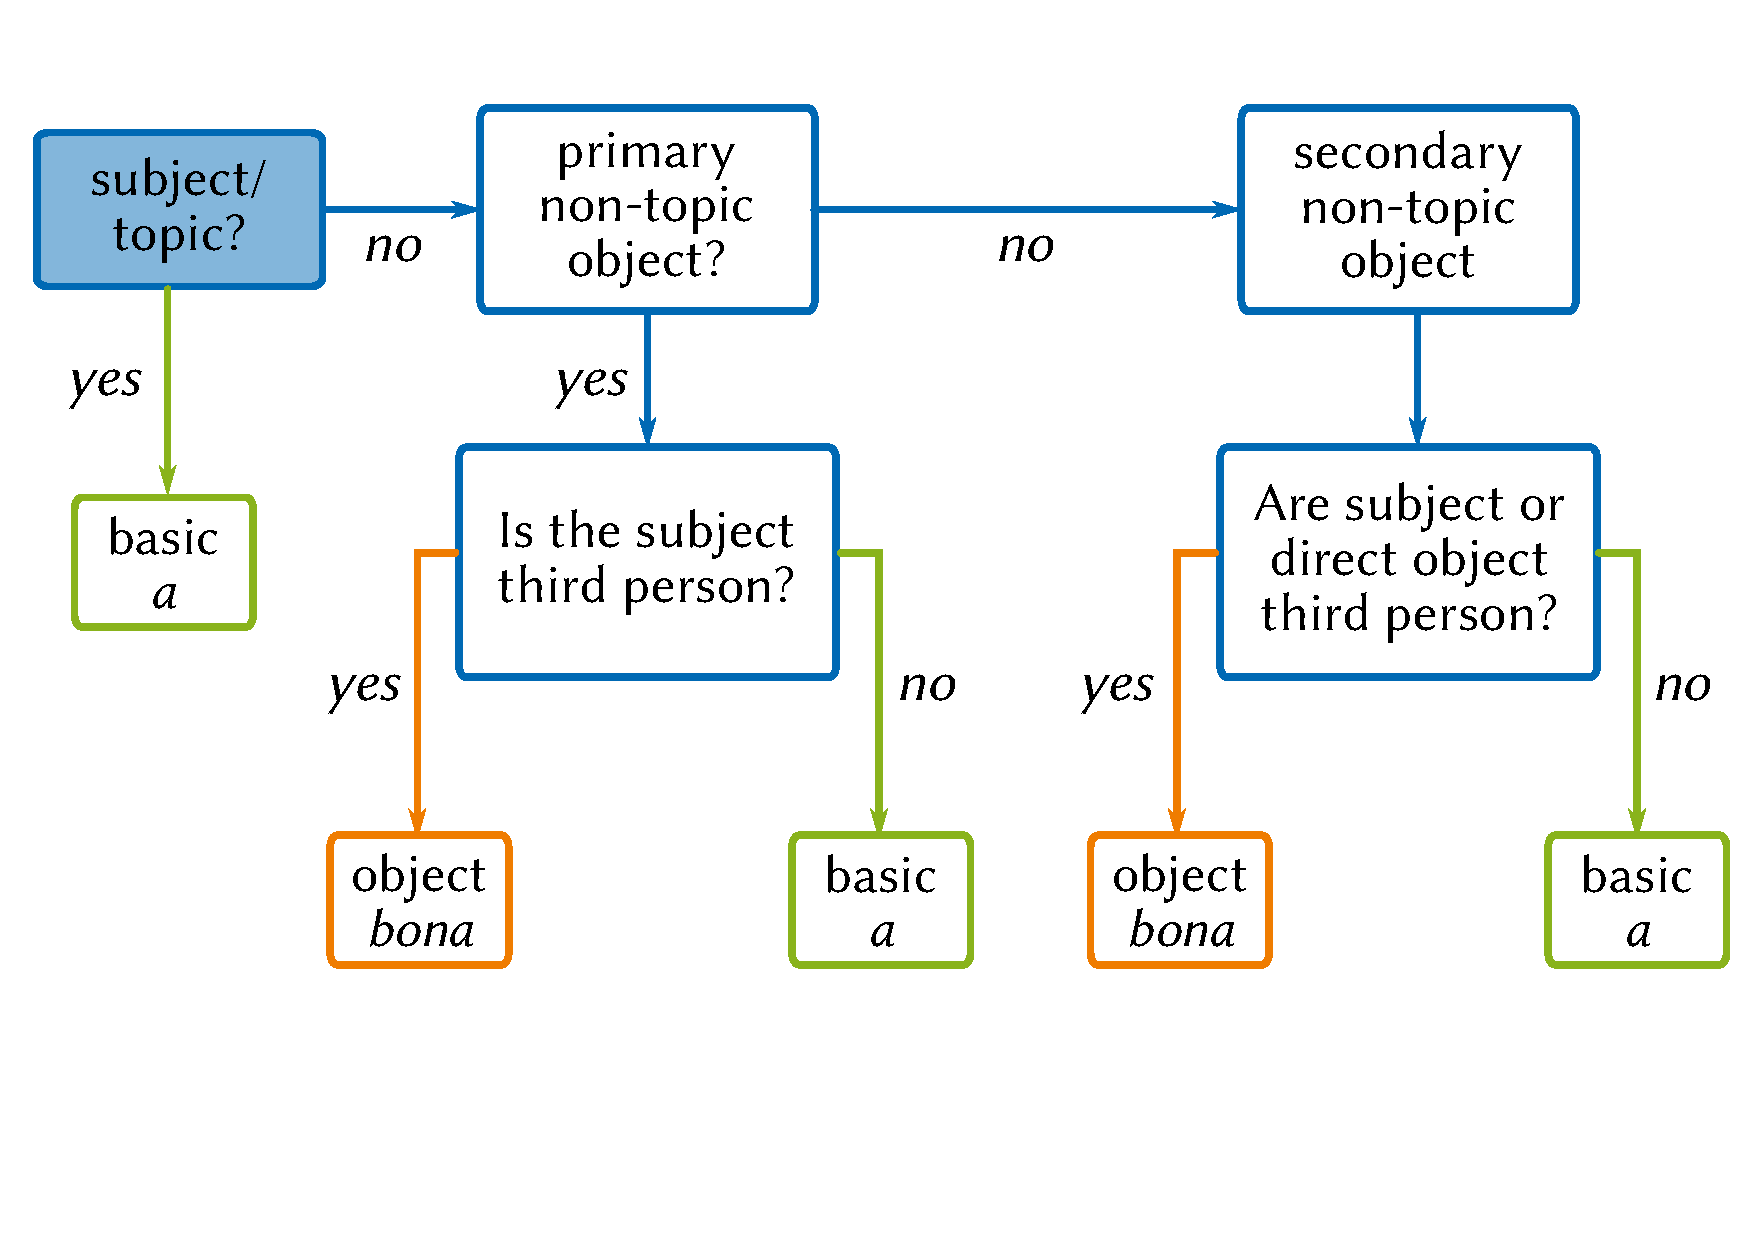
\includegraphics[width=0.7\linewidth]{TeopArgumentsFlowchart.pdf}
\caption{Actor marking in in Teop, cf. \citet{mosel2007ditransitivity}
}
\end{figure}

\citet{mosel2007ditransitivity}
\citep{mosel2007ditransitivity,greenhill2008austronesian,Forker2020}

\subsection{Syntaxtrees}

\subsubsection{X-Bar trees}

\begin{forest}
	[VP
 [DP]
 [V’
 [V]
 [DP]
 ]
 ]
	\end{forest}


\subsubsection{Transformations}

\begin{forest}
[NP [ \dots, name=dem][\ibar{N}$_1$ [DEM [ diese]] [\ibar{N}$_2$,name=nnum [ \dots, name=num] [\ibar{N}$_3$ [NUM [drei]] [\ibar{N}$_4$, name=nadj [ \dots{}, name=adj] [\ibar{N}$_5$ [ADJ [schwarzen]] [N [Hunde, name=hund]]]] ] ]]]
{\draw[->](hund)to[out=east, in=east](adj);
\draw[->](nadj)to[out=east, in=east](num);
\draw[->](nnum)to[out=east, in=east](dem);
}
\end{forest}

\subsubsection{Dependencies}

\begin{dependency}[theme = simple]
   \begin{deptext}[column sep=1em]
      The \& children \& {go} \& {to}  \& school\\
   \end{deptext}
	  % \deproot{3}{ROOT}
	   \depedge{2}{1}{1}%{det}
	   \depedge{3}{2}{1}%{subj}
	   \depedge{3}{4}{1}%{pp}
	   \depedge{4}{5}{1}%{pc}
\end{dependency}	


\subsection{Writing passages of code}

When writing passages which contain a lot of programming operators, instead of escaping each of them, use the \verb|Verbatim|-Environment to show them as they are in your console/script/notebook.

\begin{Verbatim}
ge=/.*RES.*/ &
mb
\end{Verbatim}


\subsection{References}

When using \verb|natbib|, you can specify page numbers when citing: \citep[e.g.][22]{rose2011third}.
When you may also refer to the author's name inside of your text by using \citet[33]{windfuhr2009iranian}. If you are ennumarating  multiple authors inside of a long list, you are likely wanting to avoid parantheses, in that case, use (\citealt{vydrin2018mande}, \citealt{arcodia2020morphology}).

\subsection{Quotation and Blocks}

You can add short quotes with quotation marks with \enquote{enquote, followed by the reference} \citep[4087]{Forker2020}, but you can also quote whole paragraphs in this indented format:

\begin{quote}

\lipsum[1]\citep[6]{rankin2003synchronic}

\end{quote}


\subsection{Word Count}

These are guidelines on the length of your work. Numbers are from the Department of General Linguistics and may differ for the Anglistics department. Consult your advisor:

\begin{compactitem}
\item BA: 
	\begin{compactitem}
		\item Studienarbeit: 1500-4500 Wörter
		\item Hausarbeit: 3000-6000 Wörter
	\end{compactitem}
\item MA:
	\begin{compactitem}
		\item Studienarbeit: 3000-6000 Wörter
		\item Hausarbeit: 4500-7500 Wörter
	\end{compactitem}

\end{compactitem}

INDICATE YOUR TOTAL WORD COUNT AT THE END OF YOUR WORK.
When using Overleaf and other \LaTeX-Editors, you can find the word count in the menu under Menu > Wordcount.

\section{Conclusion}
\subsection{Discussion}
\subsection{Outlook}

\bibliographystyle{authordate2} % Uses the citation style [LASTNAME, FIRSTNAME. YEAR.]
\bibliography{Bibliobraphy} % .bib file that contains your citations


\newpage

% DECLARATION OF AUTHENTICITY %%%%%%%%%%%%%%%%%%%%%%%%%%%%%%%%%%%%%%%%
% This is the declaration as used by the Gen.Ling. department, uncomment and adapt as needed, if needed

\section*{Eigenständigkeitserklärung}
\textbf{(This is the declaration as used by the Gen.Ling. department, and adapt as needed, if needed.)}
Ich versichere, dass ich die vorliegende Arbeit selbstständig verfasst und keine
anderen als die angegebenen Quellen und Hilfsmittel benutzt habe. Alle Stellen
der Arbeit, die dem Wortlaut oder dem Sinn nach anderen Werken entnommen
sind, habe ich in jedem einzelnen Fall unter Angabe der Quelle kenntlich
gemacht. Dies gilt auch für verwendete Zeichnungen, Skizzen, Ton- und
Videoaufnahmen sowie graphische Darstellungen. Ich erkläre mich damit
einverstanden, dass meine Arbeit im Verdachtsfall mithilfe einer
Plagiatssoftware überprüft wird.

\vspace{2\baselineskip}

\noindent\parbox{.45\textwidth}{\rule{.4\textwidth}{1pt}\\
Ort, Datum}
\hfill
\hfill \parbox{.45\textwidth}{\rule{.4\textwidth}{1pt}\\ Unterschrift}

\end{document}